\documentclass{beamer}
\usepackage{listings}
\usepackage{minted}
\usepackage{anyfontsize}

\mode<presentation> {
  \usetheme{Madrid}
}

\title[Robin Hood Hashing]{Missguided attempts at performance optimizations} % The short title appears at the bottom of every slide, the full title is only on the title page

\author{Radu Ciorba \href{mailto:radu@devrandom.ro}{\{radu@devrandom.ro\}}} % Your name
\date{\today} % Date, can be changed to a custom date

\begin{document}

\begin{frame}
  \titlepage % Print the title page as the first slide
\end{frame}

\begin{frame}
  \frametitle{What is Borg Backup?}
  \begin{itemize}
  \item Deduplicating backup program
  \item written mostly in python
  \item with some C code
  \item and some Cython code to tie everything together
  \end{itemize}
\end{frame}

\begin{frame}
  \frametitle{Cython you say?}
  \inputminted[fontsize=\footnotesize]{python}{snippets/example.pyx}
\end{frame}


\begin{frame}
 \begin{center}
 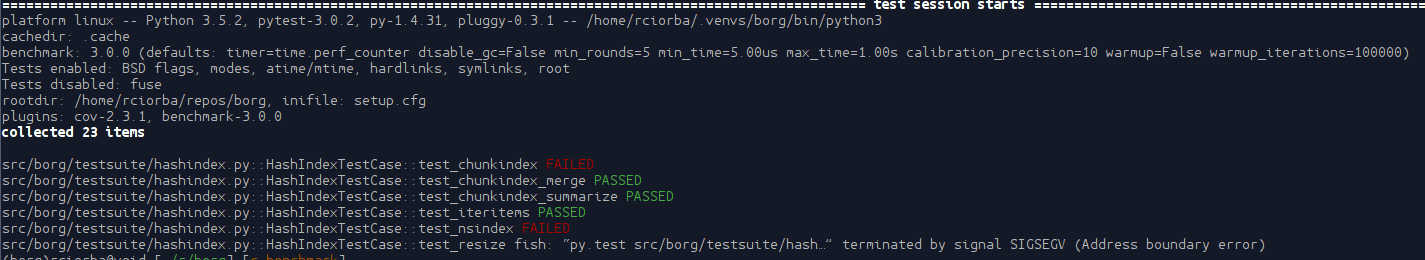
\includegraphics[scale=0.245,keepaspectratio=true]{./segfault.png}
 % excuses-for-not-writing-tests.jpg: 0x0 pixel, 300dpi, 0.00x0.00 cm, bb=
 \end{center}
\end{frame}

\begin{frame}
  \frametitle{The goal: Robin Hood hashing}
  \begin{itemize}
  \item Quick recap on hashmaps
  \item Open addressing
  \item Deletion
  \end{itemize}
\end{frame}


\begin{frame}
 \begin{center}
 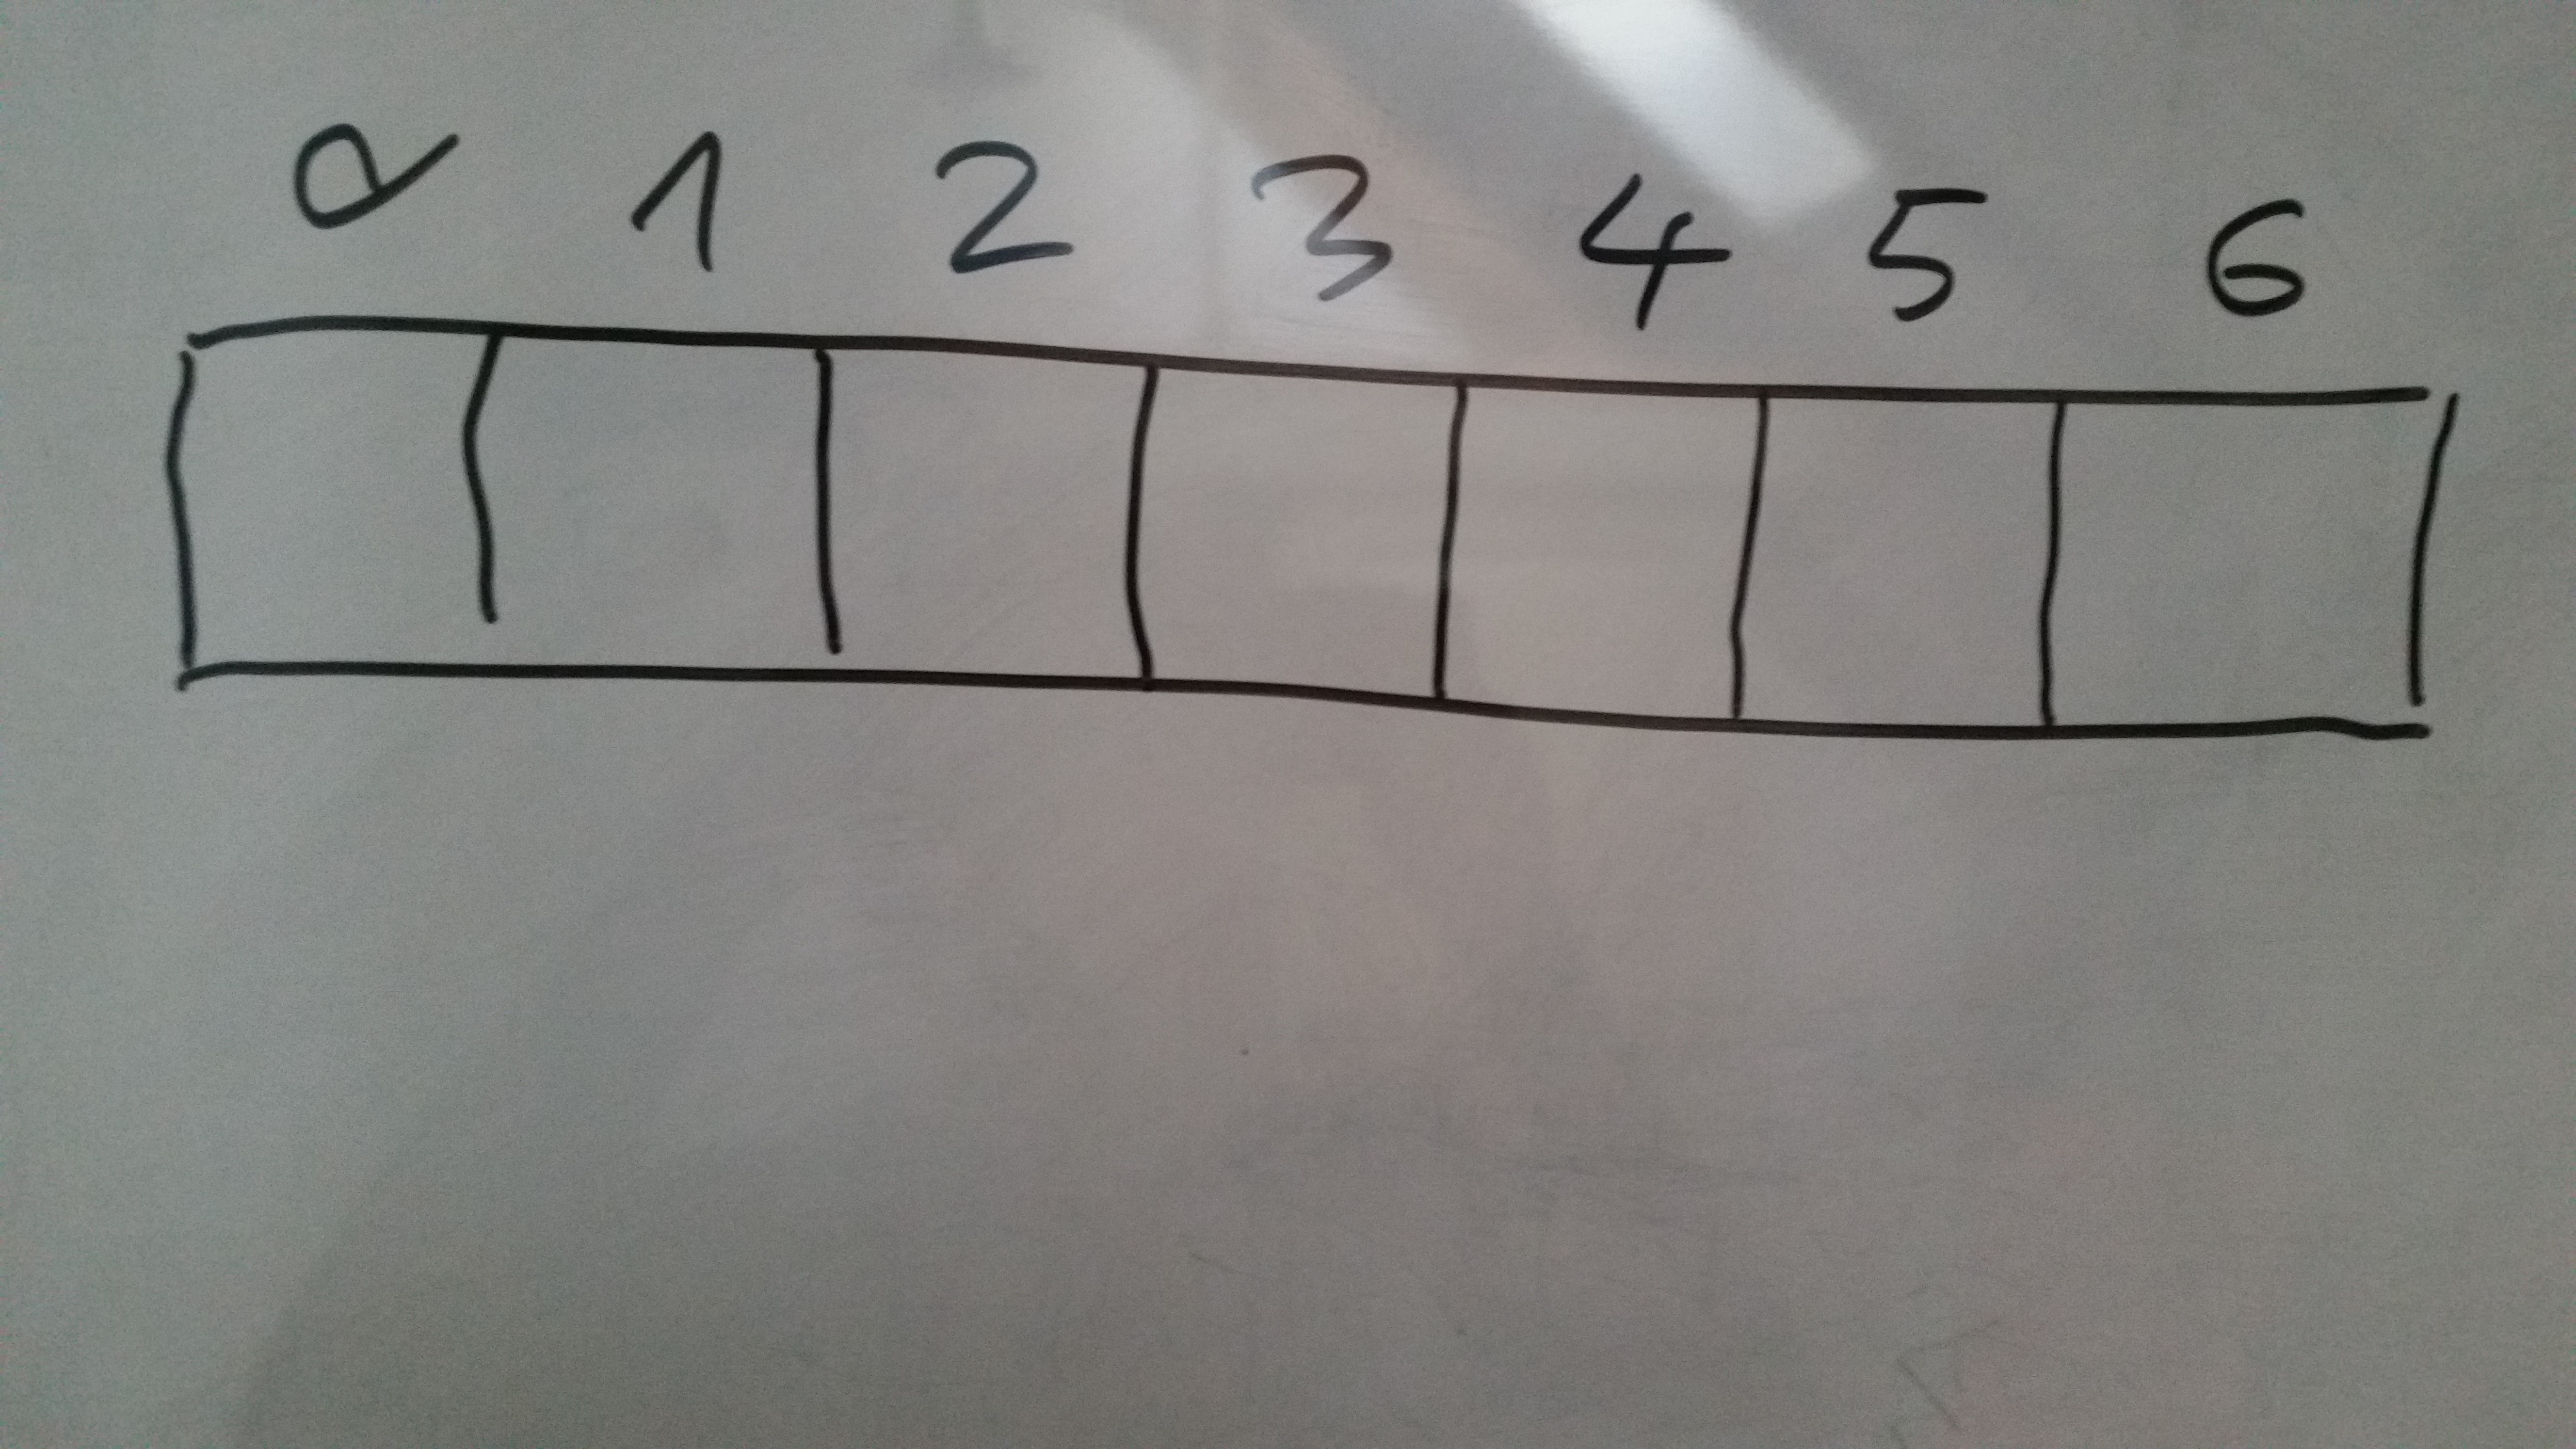
\includegraphics[scale=0.06,keepaspectratio=true]{./images/1.jpg}
 \end{center}
\end{frame}

\begin{frame}
 \begin{center}
 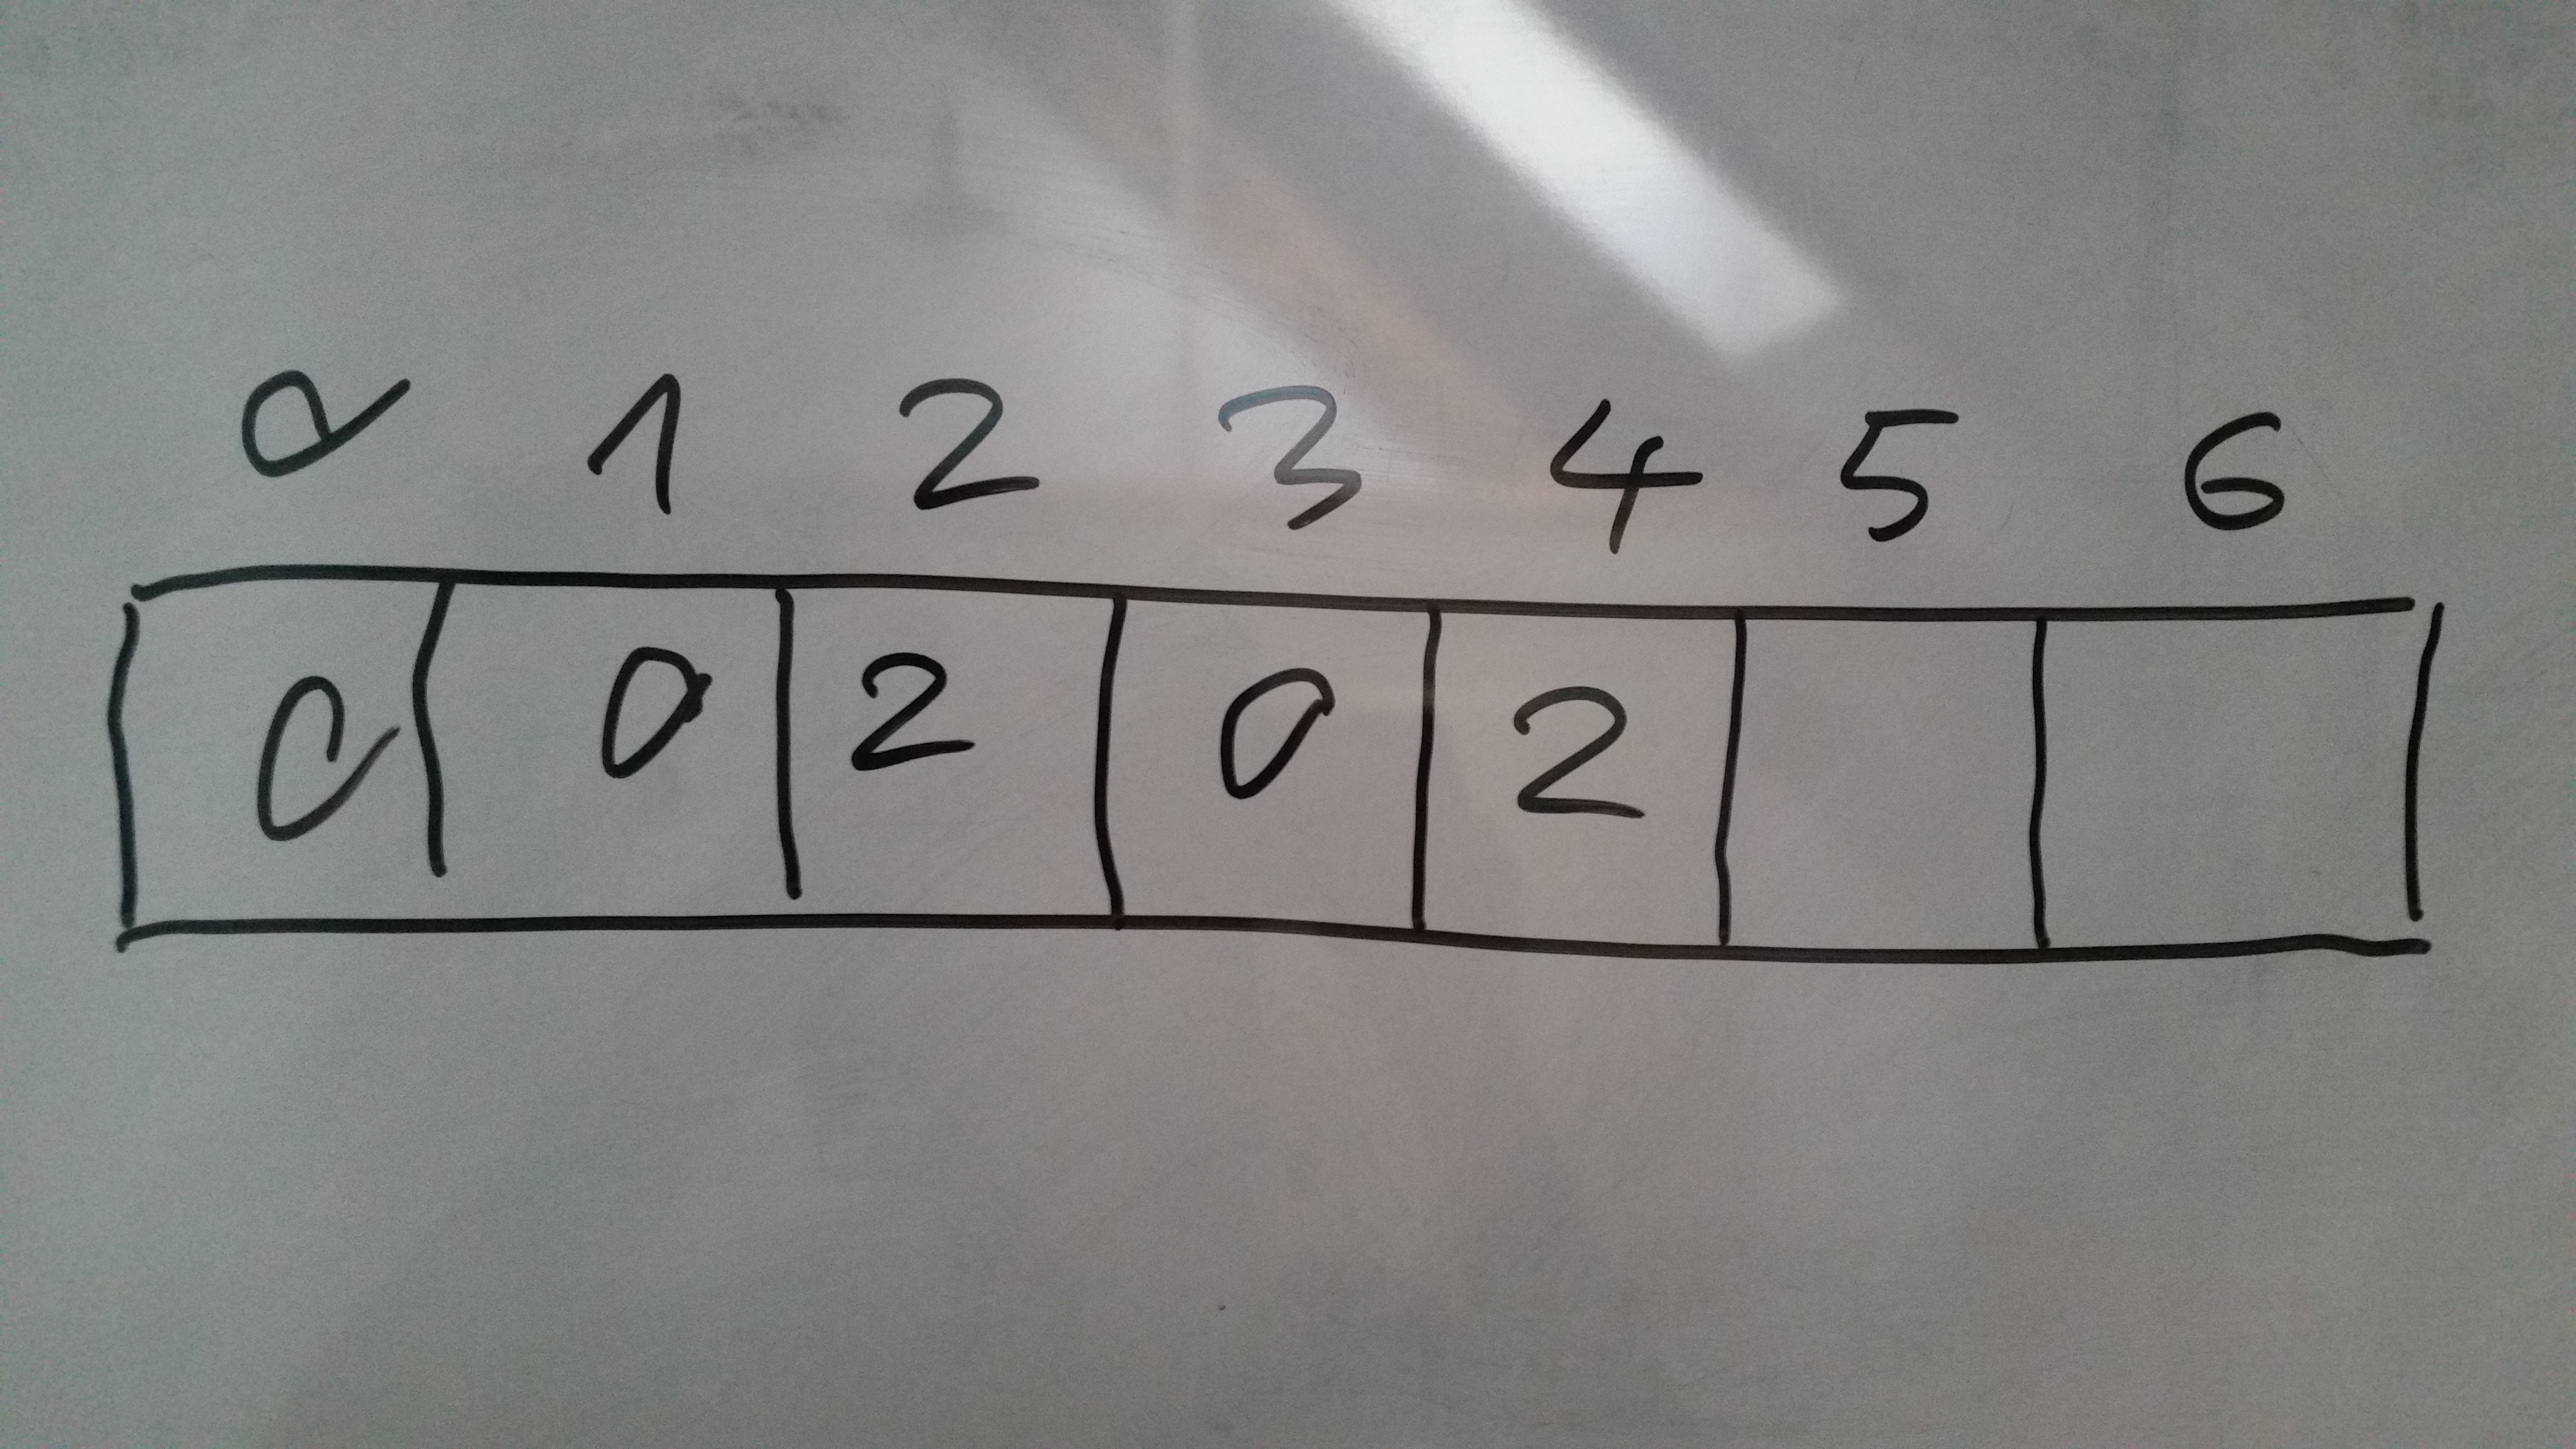
\includegraphics[scale=0.06,keepaspectratio=true]{./images/2.jpg}
 \end{center}
\end{frame}

\begin{frame}
 \begin{center}
 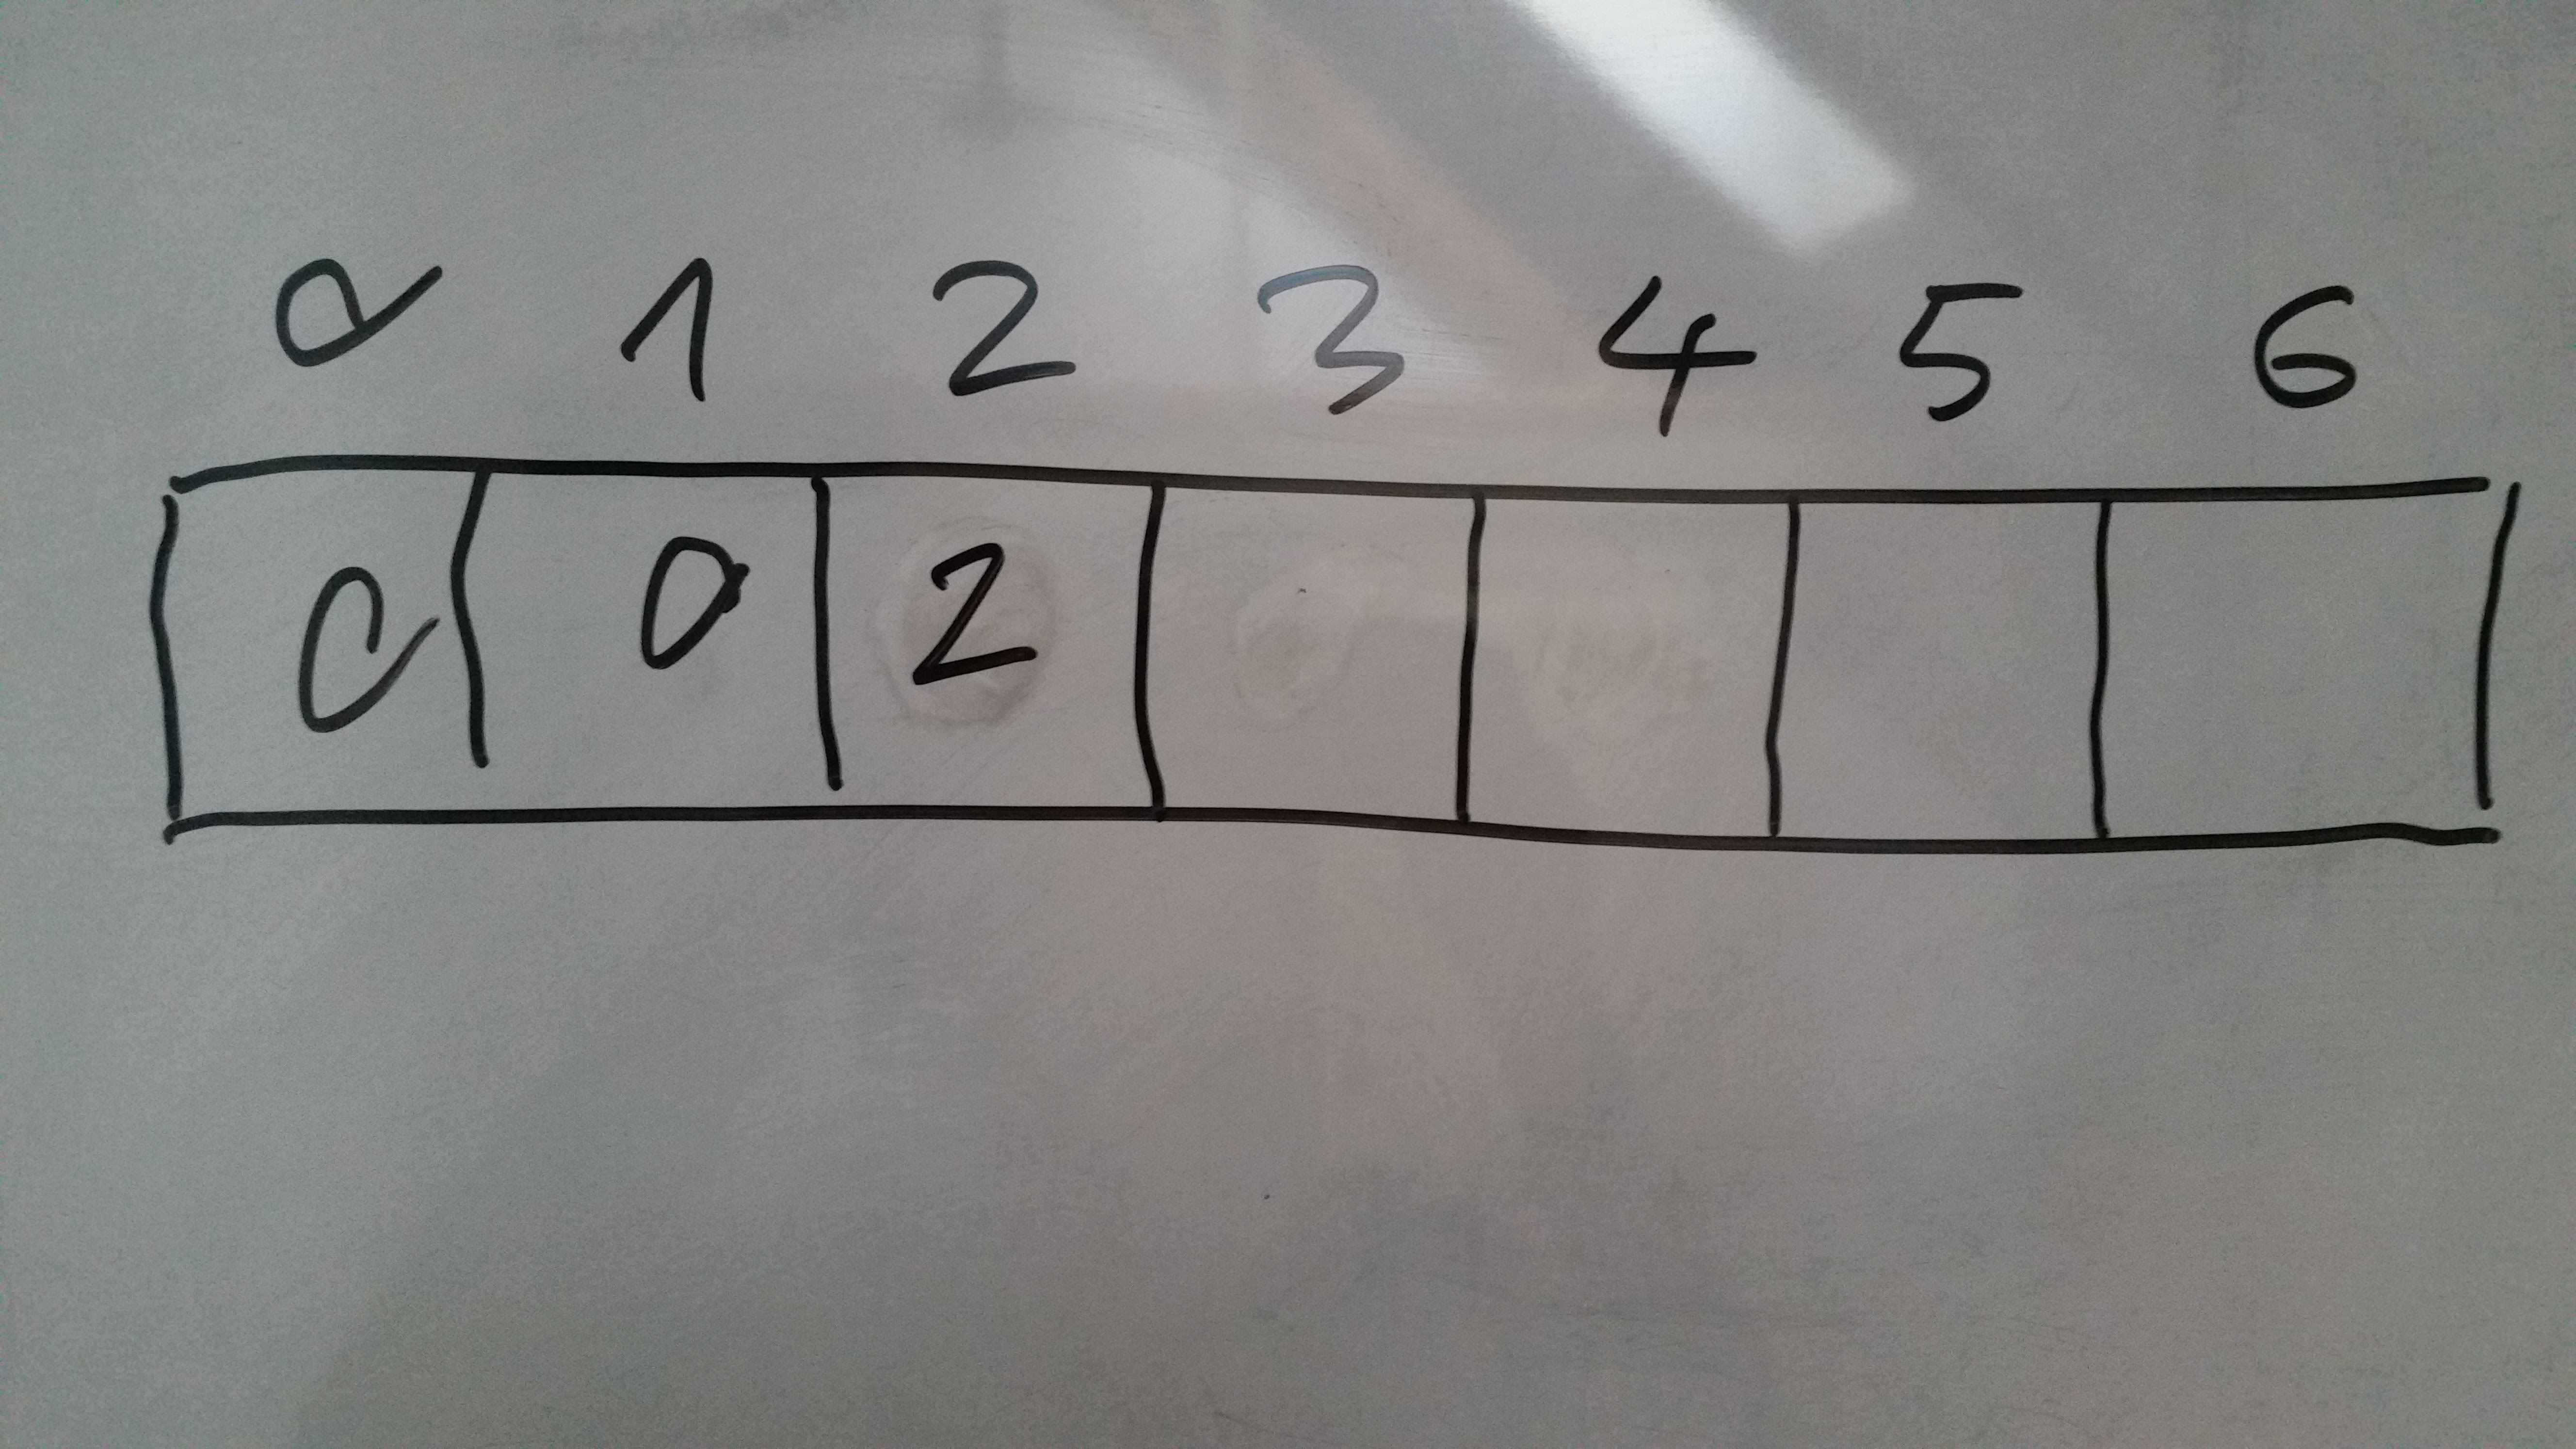
\includegraphics[scale=0.06,keepaspectratio=true]{./images/3.jpg}
 \end{center}
\end{frame}

\begin{frame}
 \begin{center}
 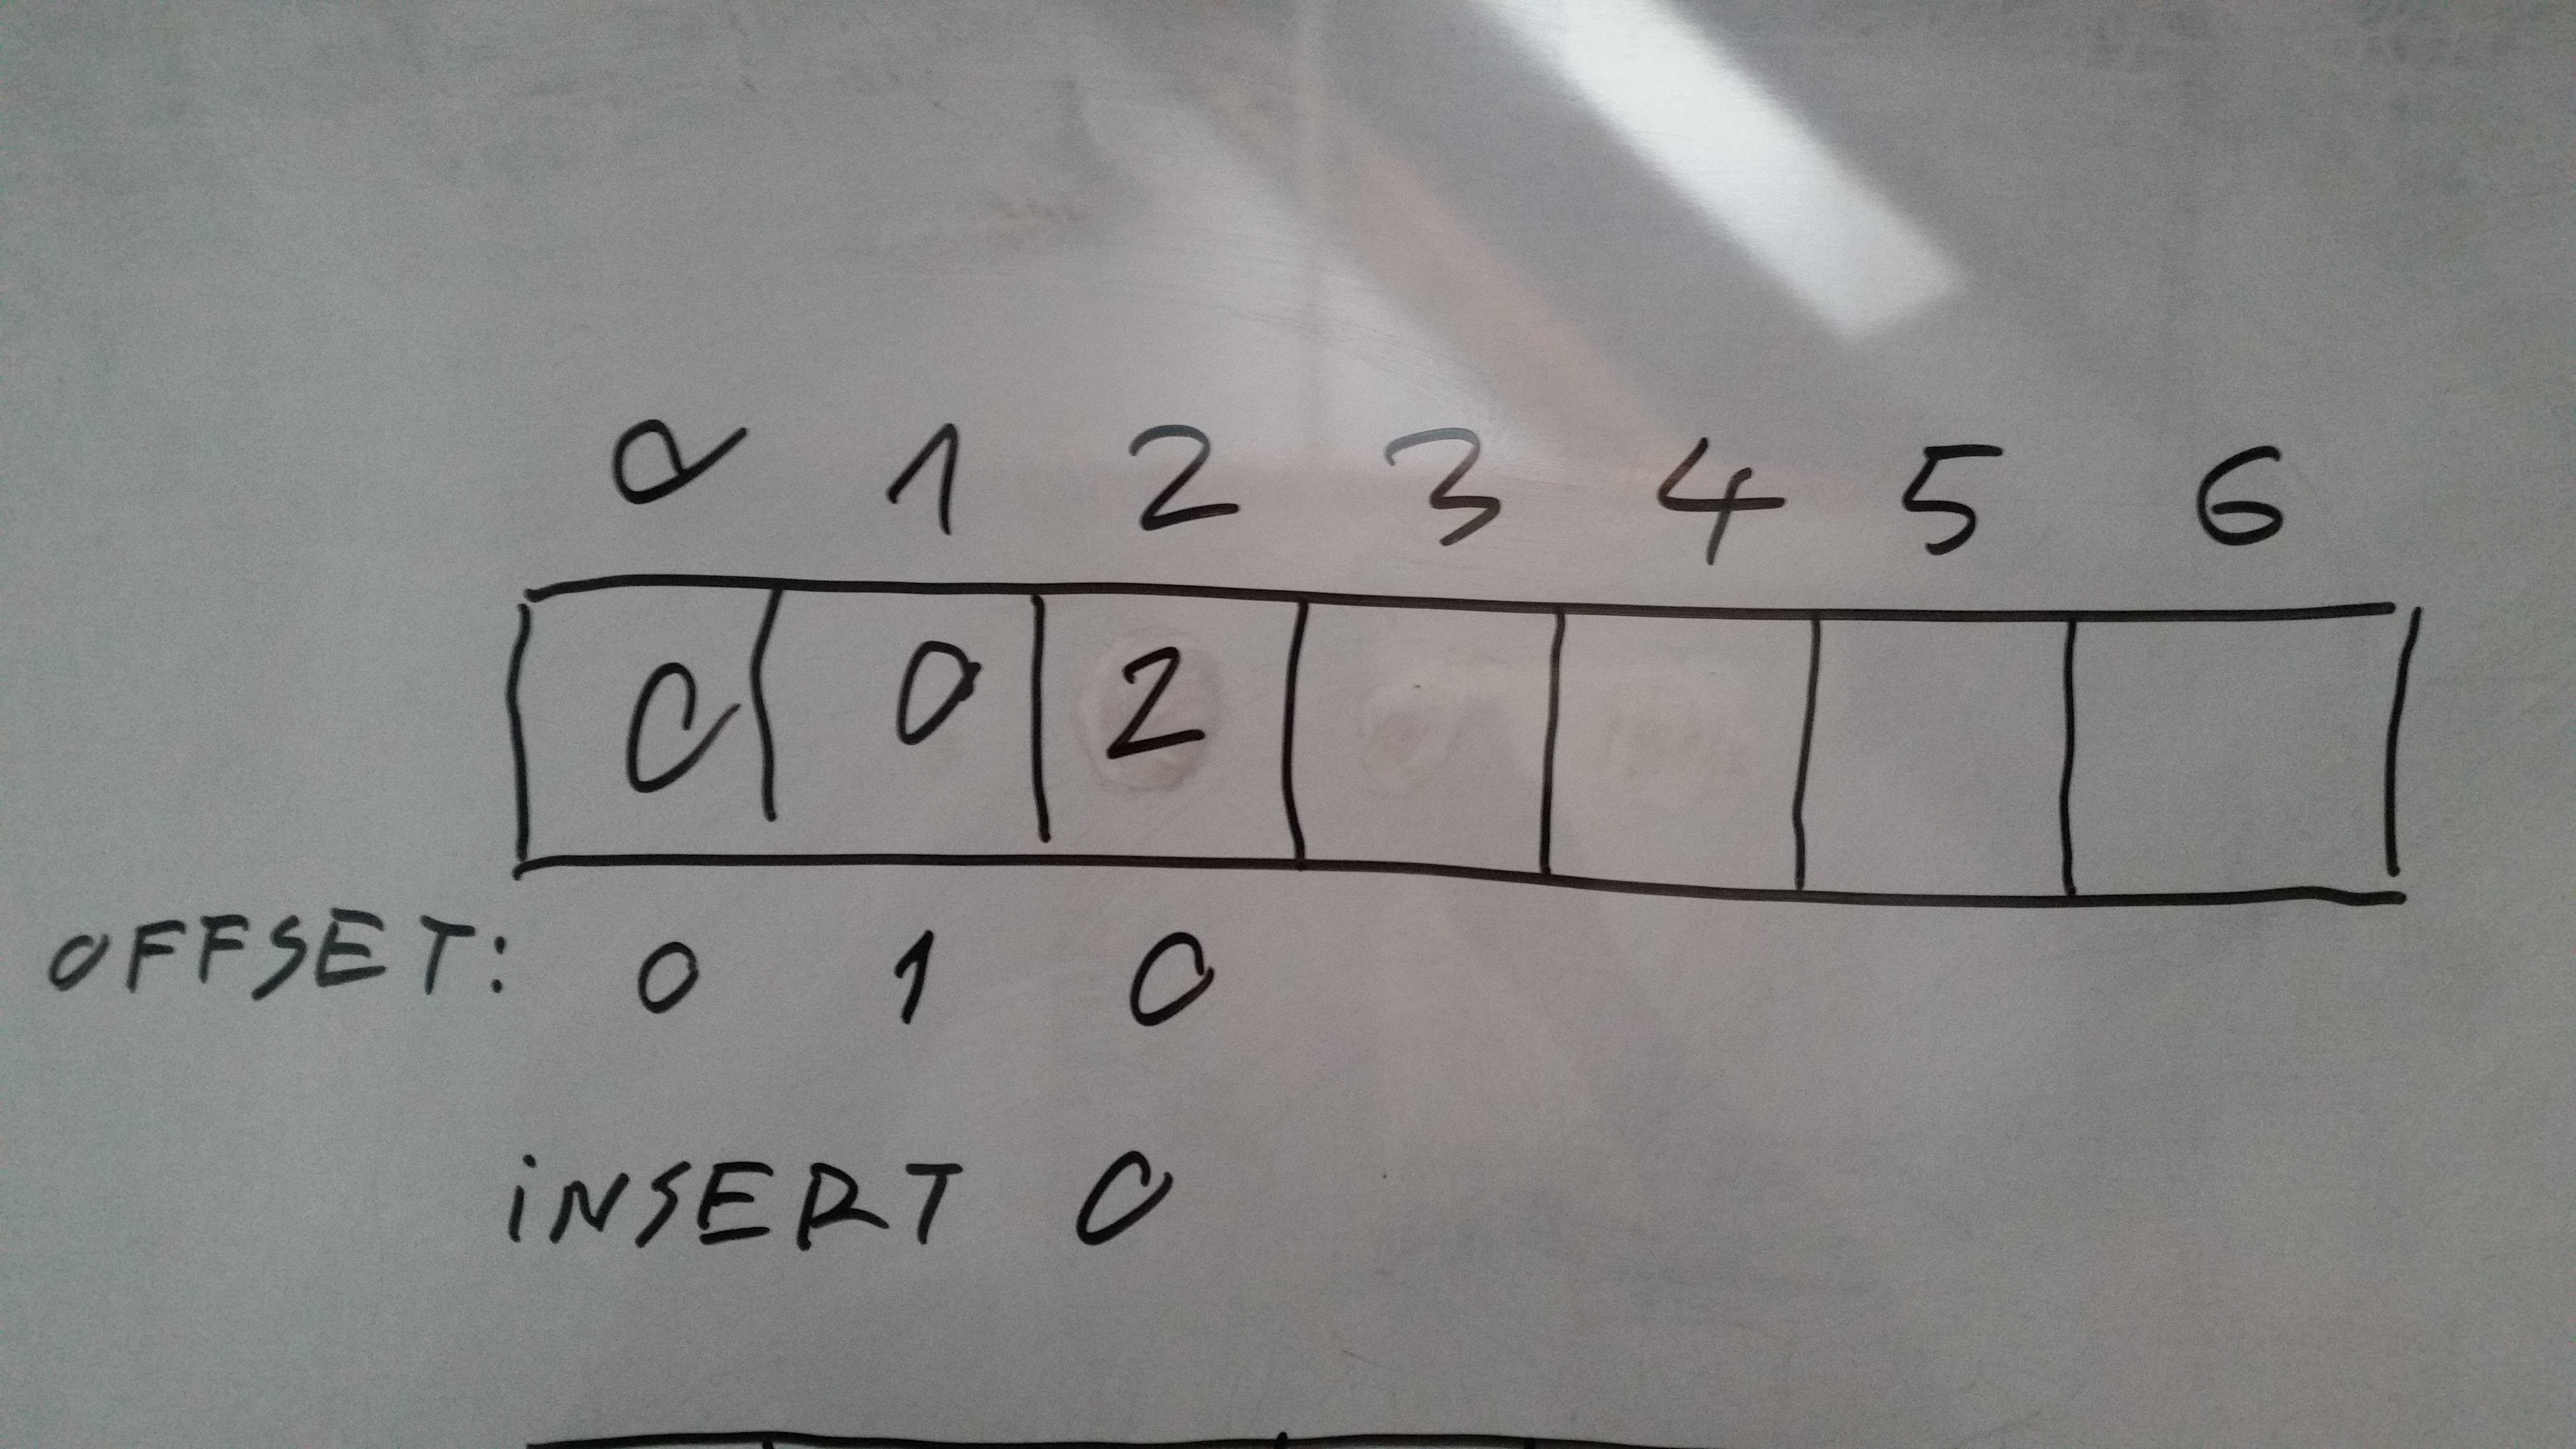
\includegraphics[scale=0.06,keepaspectratio=true]{./images/4.jpg}
 \end{center}
\end{frame}

\begin{frame}
 \begin{center}
 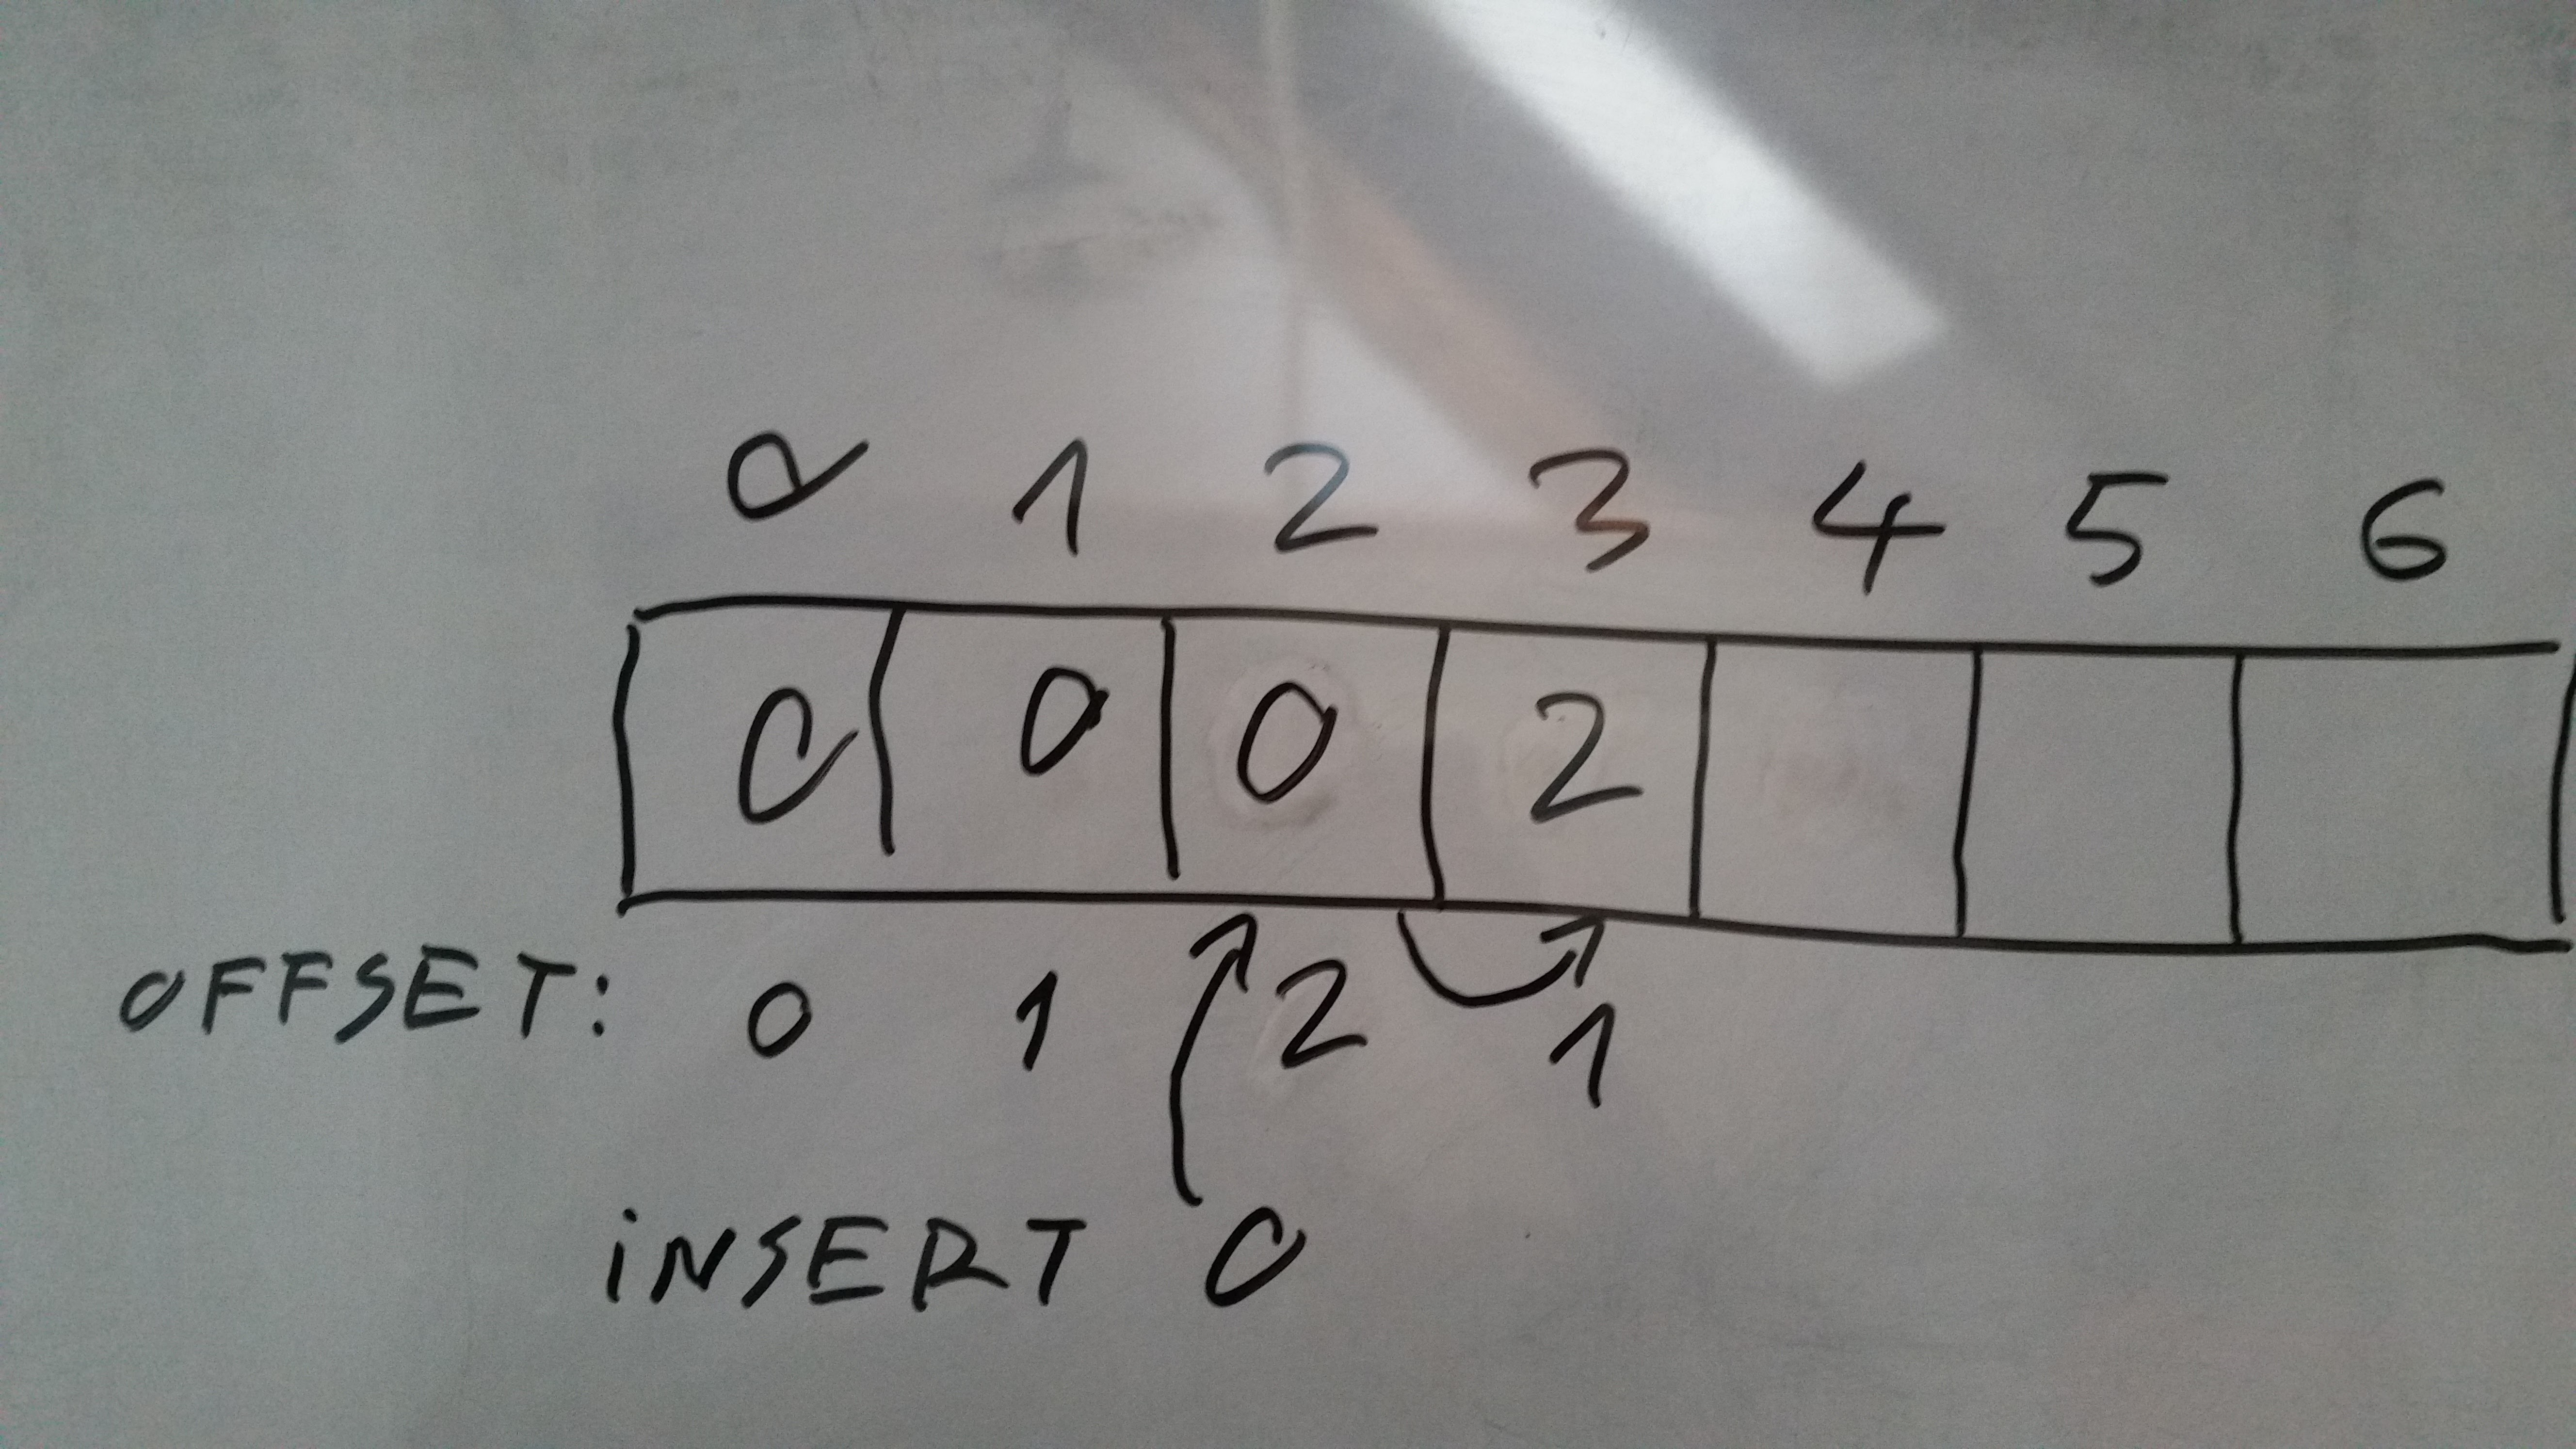
\includegraphics[scale=0.06,keepaspectratio=true]{./images/5.jpg}
 \end{center}
\end{frame}

\begin{frame}
  \frametitle{Borg's current Hash}
  \begin{itemize}
  \item key is 32 bytes, value is 12 bytes
  \item Open Addressing
  \item Tombstones
  \item hashindex\_lookup will promote buckets on top of tombstones
  \end{itemize}
\end{frame}

\begin{frame}
  insert actual implementation here ...
\end{frame}

\begin{frame}
  \frametitle{Cool story bro. Benchmarks?}
  \inputminted[fontsize=\footnotesize]{python}{snippets/bench1.py}
\end{frame}


\begin{frame}
  \frametitle{Cool story bro. Benchmarks?}
   {\fontsize{5.2pt}{5.2pt}
     \inputminted{python}{snippets/bench1.txt}
   }
\end{frame}

\begin{frame}
  \frametitle{What now?}
  \begin{itemize}
  \item RH at least faster for missing items
  \item apply more coffe + time
  \item found a bug in hashindex\_set, wasn't ever doing the position swap
  \end{itemize}
\end{frame}


\begin{frame}
  \frametitle{Repeatable benchmarks}
   {\fontsize{5.2pt}{5.2pt}
     \inputminted{python}{snippets/bench2.txt}
   }
\end{frame}
  
\begin{frame}
  \frametitle{Repeatable benchmarks}
  \begin{itemize}
  \item Use same inputs
  \item Use same machine
  \item Make sure nothing else is running
  \item CPU frequency scaling?
  \item Isolate your code as much as possible
  \end{itemize}
\end{frame}

\begin{frame}
  \frametitle{Isolated your code for testing}
  \inputminted[fontsize=\footnotesize]{python}{snippets/bench1.py}
\end{frame}

\begin{frame}
  \frametitle{Isolated your code for testing}
  \inputminted[fontsize=\footnotesize]{c}{snippets/bench.c}
\end{frame}

\begin{frame}
  \frametitle{Repeatable benchmarks}
   {\fontsize{4.5pt}{4.5pt}
     \inputminted{python}{snippets/bench3.txt}
   }
\end{frame}

\begin{frame}
  \frametitle{We need a better way to prezent these benchmarks}
\end{frame}

\begin{frame}
  \frametitle{My takeaways}
  \begin{itemize}
  \item MEASURE EVERYTHING!
  \item sometimes a 'worse' algorithm might be better
  \item integer division is slow
  \end{itemize}
\end{frame}

\begin{frame}
  \frametitle{Useful stuff}
  \begin{itemize}
  \item  \href{https://www.youtube.com/watch?v=WDIkqP4JbkE}{Scott Meyers: Cpu Caches and Why You Care}
  \item  \href{https://www.youtube.com/watch?v=vrfYLlR8X8k}{Andrei Alexandrescu: Writing Fast Code I}
  \item pytest-benchmark
  \item kcachegrind + google-perftools + https://pypi.python.org/pypi/yep
  \item A raspberry pi for running the tests

  \end{itemize}
\end{frame}

\begin{frame}
 \begin{center}
 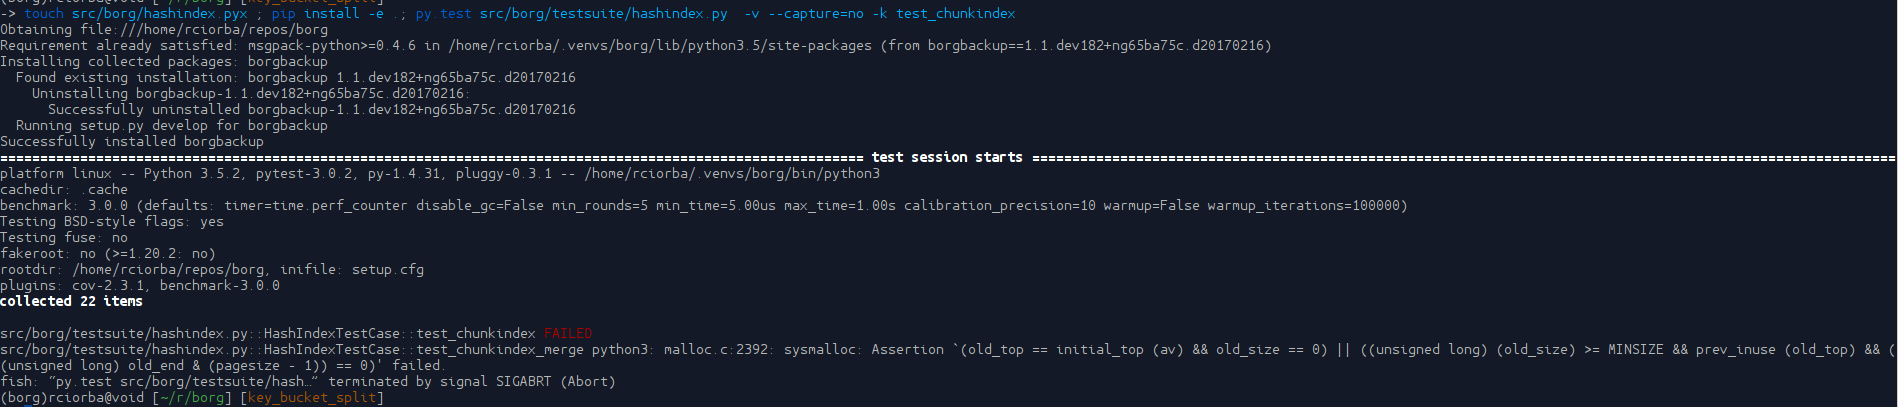
\includegraphics[scale=0.26,keepaspectratio=true]{./sigabrt.png}
 \end{center}
\end{frame}

\begin{frame}
  \frametitle{Thanks}
  You can find the code here:
  \href{https://github.com/rciorba/borgbackup}{https://github.com/rciorba/borgbackup}
  \newline
  \newline
  The slides are available at
  \href{https://devrandom.ro/talks}{https://devrandom.ro/talks}
\end{frame}

\end{document}
